\documentclass[11pt]{article}
\usepackage{geometry}                % See geometry.pdf to learn the layout options. There are lots.
\geometry{letterpaper}                   % ... or a4paper or a5paper or ... 
\usepackage{graphicx}
\usepackage{amssymb}
\usepackage{amsmath}
\usepackage{epstopdf}
\usepackage{enumerate}
\usepackage{multirow}
\usepackage{tikz}
\usepackage{pgfplots, pgfplotstable}
\usepackage{url}
\usepackage{wrapfig}
\DeclareGraphicsRule{.tif}{png}{.png}{`convert #1 `dirname #1`/`basename #1 .tif`.png}


\makeatletter
\long\def\ifnodedefined#1#2#3{%
    \@ifundefined{pgf@sh@ns@#1}{#3}{#2}%
}

\pgfplotsset{
    discontinuous/.style={
    scatter,
    scatter/@pre marker code/.code={
        \ifnodedefined{marker}{
            \pgfpointdiff{\pgfpointanchor{marker}{center}}%
             {\pgfpoint{0}{0}}%
             \ifdim\pgf@y>0pt
                \tikzset{options/.style={mark=*, fill=white}}
                \draw [densely dashed] (marker-|0,0) -- (0,0);
                \draw plot [mark=*] coordinates {(marker-|0,0)};
             \else
                \tikzset{options/.style={mark=none}}
             \fi
        }{
            \tikzset{options/.style={mark=none}}        
        }
        \coordinate (marker) at (0,0);
        \begin{scope}[options]
    },
    scatter/@post marker code/.code={\end{scope}}
    }
}

\makeatother

\textheight = 9 in
\textwidth = 6.5 in
\oddsidemargin 0 in

\title{
\vspace{-20.mm}
CS57300: Homework 1 Solution}
\author{Due date: Sunday February 1, midnight (submit pdf to Blackboard)}
\date{}                                           % Activate to display a given date or no date

\begin{document}
\maketitle

\vspace{-5.mm}
\noindent  \emph{Submit both your answers to the questions and the R code that you used for analysis. Your homework must be typed and submitted as a PDF. Use of Latex is recommended, but not required. }
\vspace{2.mm}


\section{Counting (2 pts)}


\begin{enumerate}[(a)]
	\item 
		\begin{enumerate}[(1)]
		\item $36^6 + 36^7 +36^8+36^9+36^{10} \approx 3.76 * 10^{15}$
		\item $92^6 + 92^7 +92^8+92^9+92^{10} - 82^6 - 82^7 -82^8 - 82^9-82^{10} \approx 3.0 * 10^{19}$
		\end{enumerate}
	
	\item 
		\begin{enumerate}[(1)]
		\item $92^6 + 92^7 +92^8+92^9+92^{10} \approx 4.39 * 10^{19}$
		\item $\sum_{n=6}^{10} 92^n -82^n-66^n-62^n+10^n+26^n+30^n$
		\end{enumerate}
\end{enumerate}

\section{Axioms of probability (2 pts)}

\begin{enumerate}[(a)]
  \item $P(A \cup B) = P(A) +P(B \setminus (A \cap B)) \Rightarrow P(B \setminus (A \cap B)) =  P(A \cup B) - P(A)$ 
  \\ $P(B) = P(B \setminus(A \cap B)) + P(A \cap B) \Rightarrow P(B \setminus (A \cap B)) = P(B) - P(A \cap B)$
  \\Then we can get:
  \\$P(A \cup B) - P(A) = P(B) - P(A \cap B)$
  \\$P(A \cup B) = P(A)+ P(B) - P(A \cap B)$
  	
  \item $P(B|A,C) = \frac{P(A,B,C)}{P(A,C)} $ \\ 
  		$= \frac{P(A|B,C)P(B,C)}{P(A|C)P(C)}  $  \\
  		$=\frac{P(A|B,C)P(B|C)P(C))}{P(A|C)P(C)}$\\
  		$= \frac{P(A|B,C)P(B|C))}{P(A|C)}$
\end{enumerate}


\section{Probability and conditional probability (3 pts)}
\begin{enumerate}[(a)]
  \item 
  \begin{enumerate}[(i)]
  	\item $P($ at least once$) = P( $fail at first time $) = 2 / 8 = 1/4$
 	\item $P($ at most twice$) = P( $fail at first time $) * P($ success at second time $) = \frac{2}{8} * \frac{6}{8} 	= \frac{3}{16}$
  \end{enumerate}  
  \item  There are 15 case that Alice win the game, if Alice want to win with number, the other number will only by 1,2,3,4, so the probability Alice won, and she rolled a 5 is 4/15.
\end{enumerate}


\section{Probability distributions (3 pts)}




\begin{enumerate}[(a)]
  \item 
  	\begin{tabular}{ c c c c c c }
  		$F(x)$ & 1 & 2 & 3 & 4\\ \hline 
  				& 0.1 & 0.3 &0.6&1
	\end{tabular}\\
  	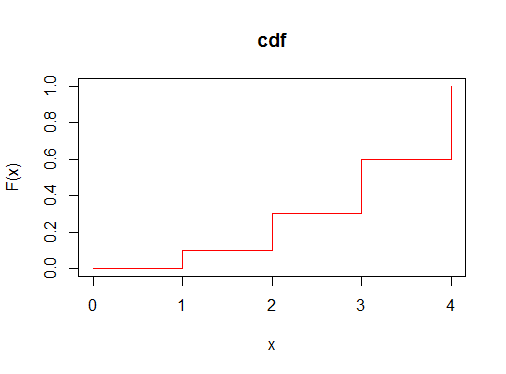
\includegraphics[width=4in]{cdf.png}
  \item 
	\begin{tabular}{ c c c c c c }
  		$p(x)$ & 1 & 2 & 3 & 4\\ \hline 
  				& 0.1 & 0.2 &0.3&0.4
	\end{tabular}  \\
    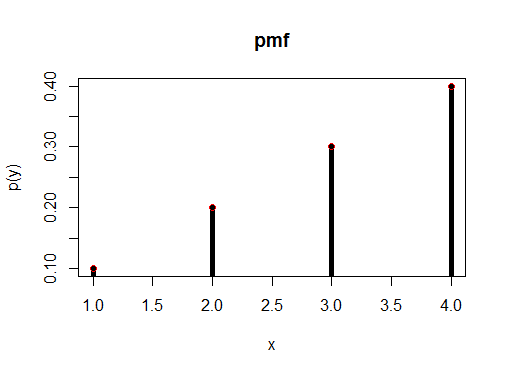
\includegraphics[width=4in]{pmf.png}
  \item $E(X) = 1*0.1 +2*0.2 +3*0.3 + 4*0.4 = 3$\\
  $Var(X) = (1-3)^2*0.1 + (2-3)^2*0.2 + (3-3)^2*0.3+(4-3)^2*0.4 = 1$
\end{enumerate}


\section{Independence (3 pts)}

\begin{enumerate}[(a)]
  \item No. Because disk 1 is red and green.
  \item No. Because disk 4 is green and white
  \item Green and black, white and black
  \end{enumerate}

\section{Conditional Expectation (2 pts)}

According p(x,y)=48/(45xy),we get $P(x=2,y=4)=2/15$ ,$P(x=2,y=1)= 8/15$, $P(x = 4,y =1) = 4/15$, $P(x=4,y=4) = 1/15$.\\
According total probability  $P(x=2)= P(x=2,y=4) + P(x=2,y=1) = 10/15 = 2/3$, $P(x=4) = P(x = 4,y =1) + P(x=4,y=4) = 5/15=1/3$ \\
so $P(y = 1|x=2) = P(x=2,y=1) / P(x=2) = 4/5$ \\
$P(y = 4|x=2) = P(x=2,y=4) / P(x=2) = 1/5$\\
$P(y = 1|x=4) = P(x=4,y=1) / P(x=4) = 4/5$\\
$P(y = 4|x=4) = P(x=4,y=4) / P(x=4) = 1/5$\\
$E(Y|x=2) = 1 * P(y= 1|x=2) +  4*P(y=4|x=2) = 4/5 + 4*1/5 = 8/5$\\
$E(Y|x=4) = 1 * P(y= 1|x=4) +  4*P(y=4|x=4) = 4/5 + 4*1/5 = 8/5$\\
$E(Y^2|x=2) = 1 * P(y= 1|x=2) +  4^2*P(y=4|x=2) = 4/5 + 16*1/5 = 4$\\
$E(Y^2|x=4) = 1 * P(y= 1|x=4) +  4^2*P(y=4|x=4) = 4/5 + 16*1/5 = 4$\\
$Var(Y|x=2) = 4 - (8/5)^2 = 1.44$\\
$Var(Y|x=4) = 4 - (8/5)^2 = 1.44$

\section{Correlation (5 pts)}

\begin{enumerate}[(a)]
\item 
\item Both covariance and correlation are described how two variables related, but correlation standardizes covariance by dividing through standard deviation. $Corr(X,Y) = 1$ represent two variables positive related perfectly, but $Cov(X,Y) = 1$ represent two variables are positive related but not so perfectly. So $corr(X,Y)= 1$ will be more stronger. 
\item Based on Proposition: $Cov(X,Y)= E(XY)-E(X)E(Y)\\
Cov(aX+b,cY+d) = E((aX+b)(cY+d))-E(aX+b)E(cY+d)=E(acXY+bcY+adX+bd) - E(aX+b)E(cY+d)=acE(XY)+bcE(Y)+adE(X)+E(bd)- (aE(X)+b)(cE(Y)+d) = acE(XY)+bcE(Y)+adE(X)+E(bd) - (acE(X)E(Y)+adE(X)+bcE(Y)+E(bd)) = acE(XY)-acE(X)E(Y) = acCov(X,Y)$\\
$Corr(aX+b,cY+d) = \frac{Cov(aX+b,cY+d)}{\sqrt {Var(aX+b)}* \sqrt{ Var(cY+d)}} = \frac{acCov(X,Y)}{\left | a \right | \left | c \right | \sqrt{Var(X)Var(Y)}}$\\
Therefore if a,and c are opposite, $Corr(aX+b,cY+d)= -Corr(X,Y)$ and $Cov(aX+b,cY+d) = acCov(X,Y)$
\end{enumerate}

%\newpage
\section{Exploratory Data Analysis (15 pts)}
\subsection*{R Questions}
\begin{enumerate}[(a)]
\item 
Plot a histogram of the \texttt{tip\_count} attribute. Use the \texttt{hist()} function with its default values and make sure to title the plot with the name of the attribute for clarity. Next plot a histogram using the log values of tip\_count.\\

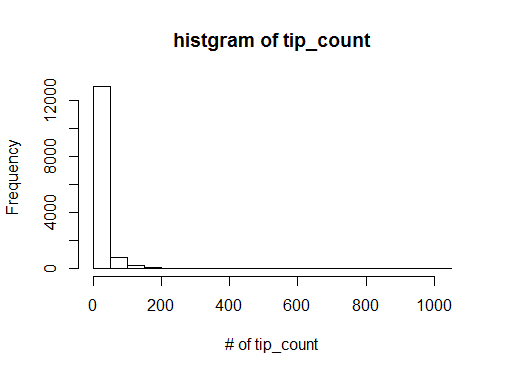
\includegraphics[width=4in]{tip_count.png}\\
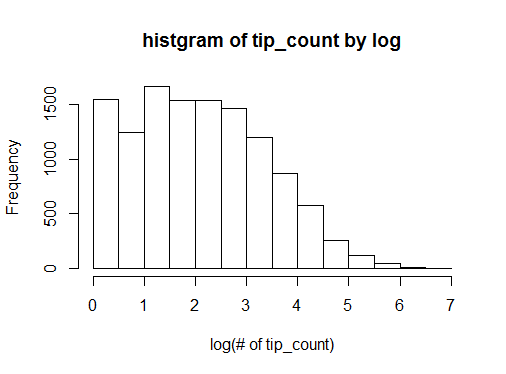
\includegraphics[width=4in]{tip_count_log.png}

\item 
Plot the \texttt{tip\_count} attribute again but this time use the \texttt{density()} function in the plot, for both the original and the logged values.\\
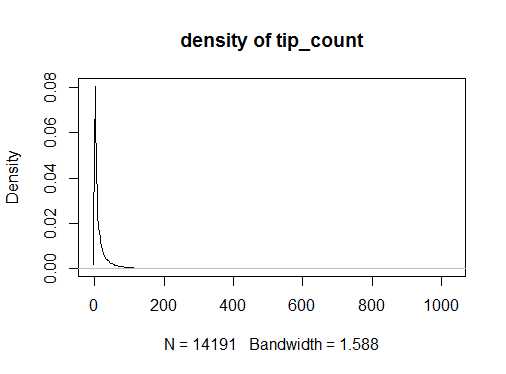
\includegraphics[width=4in]{density.png}\\
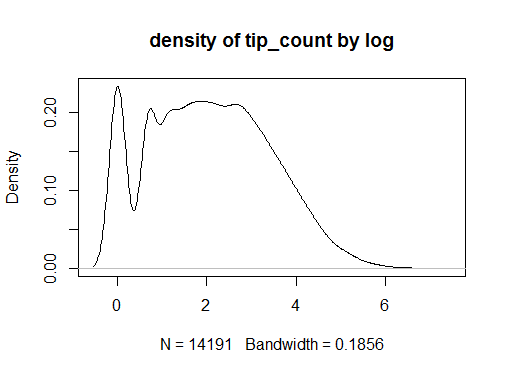
\includegraphics[width=4in]{density_log.png}


\item 
Find the continuous attribute with \textbf{largest} range and plot a histogram of the values. 
Make sure to title the plot with the name of the attribute for clarity.\\
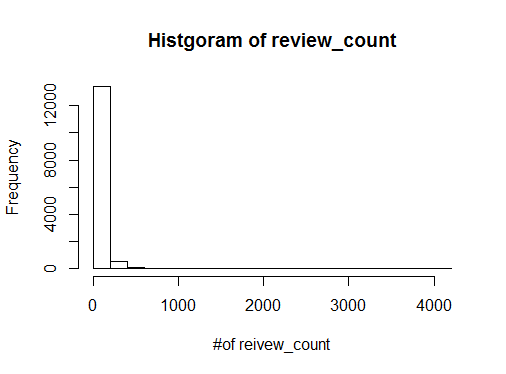
\includegraphics[width=4in]{largestrange.png}


\item 
Find the discrete attribute (that is not a unique identifier) with the \textbf{maximum} number of values and plot a barplot to show the frequency of each value. 
Note that this will look like a histogram but for nominal values. Again, make sure to title the plot with the name of the attribute for clarity.\\
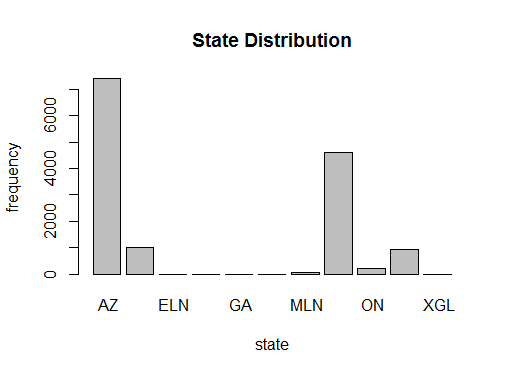
\includegraphics[width=4in]{barplot_discrete.png}


\item  
Consider the four continuous attributes: \texttt{latitude, longitude, stars, likes}. Calculate the pairwise correlations among these four attributes. 
Plot scatterplots for the pair of attributes with largest positive correlation and the pair of attributes with largest negative correlation. 
Make sure to label both axis of the plot with the attribute names. Report the correlations and discuss whether the correlations are interesting or expected, given your domain knowledge.\\
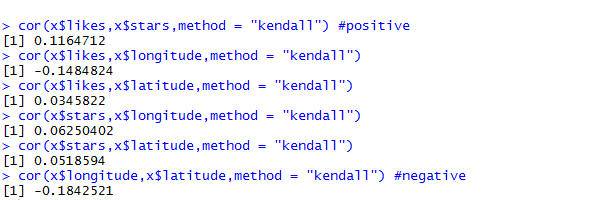
\includegraphics[width=4in]{cor_result.png} \\
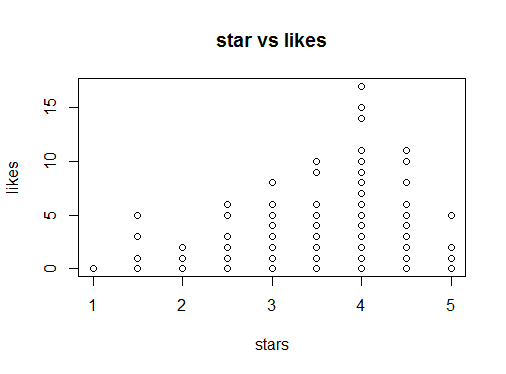
\includegraphics[width=4in]{star vs likes.png} \\
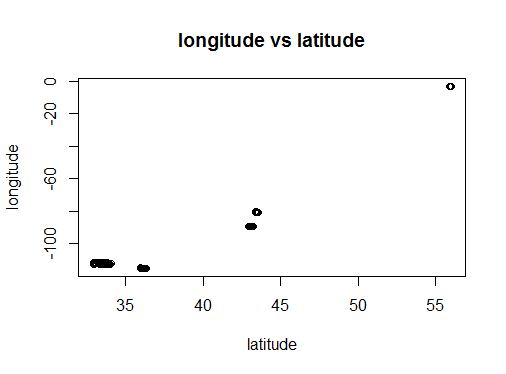
\includegraphics[width=4in]{longitude vs latitude.png}\\
stars and likes has positive correlation, it is because if people like the restaurant, they will rate higher stars for that restaurant.
\item  
Choose a particular category (e.g., Nightlife) and create a new binary feature for each example that records whether the example contains the chosen category (e.g., Nightlife vs. not-Nightlife). You can use the \texttt{regexpr()} function to test whether the list contains a particular string. Plot a boxplots of your new binary feature vs. stars and likes (i.e., {\em feature vs. stars} and {\em feature vs. likes}).
Make sure to label both axes of the plot with the attribute/feature names.\\
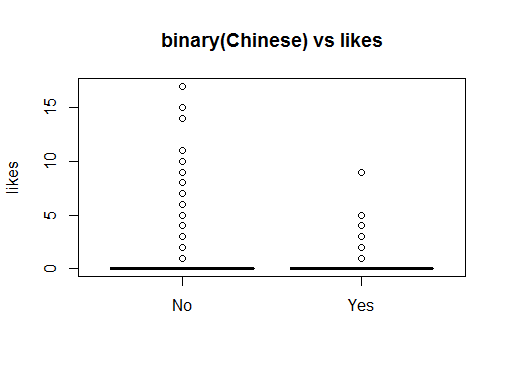
\includegraphics[width=4in]{boxplot_likes.png}\\
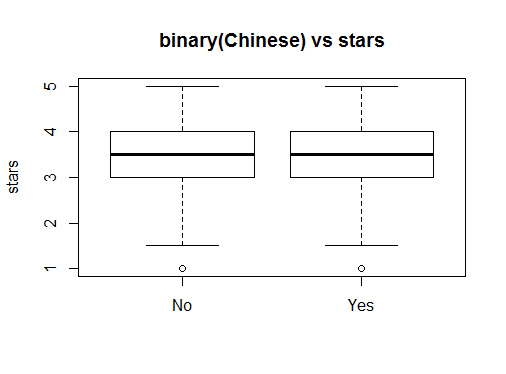
\includegraphics[width=4in]{boxplot_stars.png}
\item 
Continue with the same approach you used above to explore several categories (e.g., {\em Bars, Diners}).  Construct at least two new binary features from those categories  that exhibit a difference in the star ratings (between categories). Plot the boxplots and discuss whether the relationship is interesting or expected, given your domain knowledge.\\
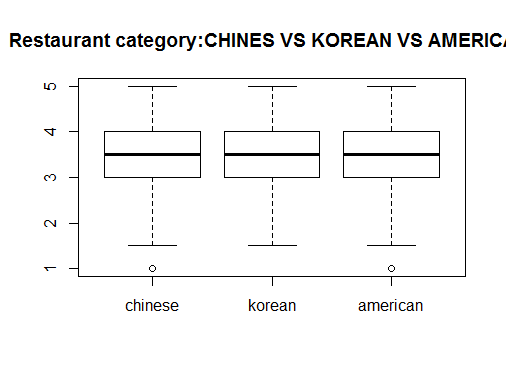
\includegraphics[width=4in]{multiple.png}\\
According the boxplot, we can conclude that the korean restaurant, american restaurant,and chinese restaurant are all relative good, because they have similar score. That's can proved by those type of restaurants are very easy to find in our life. 
\end{enumerate}
\end{document}  



